\begin{figure}[H]
    \centering
    \begin{subfigure}{\ResultSubFigureWidth \linewidth}
        \centering
        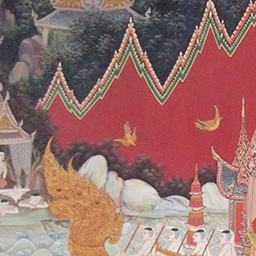
\includegraphics[width=\ResultSubFigurePadding \linewidth]{image/thaiart/case01-original.png}
        \caption{วัดแก้วไพฑูรย์}
        \label{image:thaiart_case01_original}
    \end{subfigure}
    \begin{subfigure}{\ResultSubFigureWidth \linewidth}
        \centering
        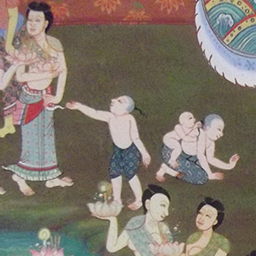
\includegraphics[width=\ResultSubFigurePadding \linewidth]{image/thaiart/case02-original.png}
        \caption{วัดแก้วไพฑูรย์}
        \label{image:thaiart_case02_original}
    \end{subfigure}
    \begin{subfigure}{\ResultSubFigureWidth \linewidth}
        \centering
        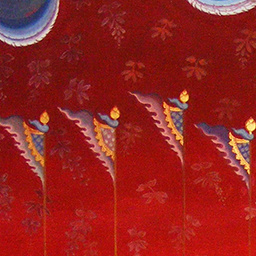
\includegraphics[width=\ResultSubFigurePadding \linewidth]{image/thaiart/case03-original.png}
        \caption{วัดพระยืนพุทธบาทยุคล}
        \label{image:thaiart_case03_original}			
    \end{subfigure}		
    \begin{subfigure}{\ResultSubFigureWidth \linewidth}
        \centering
        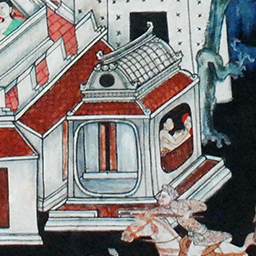
\includegraphics[width=\ResultSubFigurePadding \linewidth]{image/thaiart/case04-original.png}
        \caption{วัดคงคาราม}
        \label{image:thaiart_case04_original}			
    \end{subfigure}
    \begin{subfigure}{\ResultSubFigureWidth \linewidth}
        \centering
        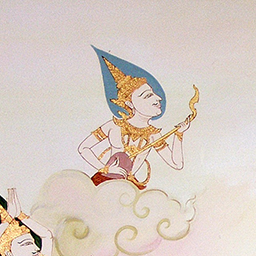
\includegraphics[width=\ResultSubFigurePadding \linewidth]{image/thaiart/case05-original.png}
        \caption{วัดท่าถนน}
        \label{image:thaiart_case05_original}			
    \end{subfigure}
    \begin{subfigure}{\ResultSubFigureWidth \linewidth}
        \centering
        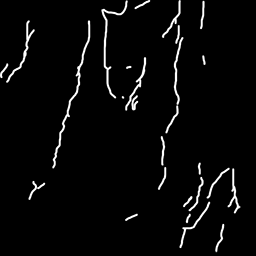
\includegraphics[width=\ResultSubFigurePadding \linewidth]{image/thaiart/inpaint-domain.png}
        \caption{รอยความเสียหาย}
    \end{subfigure}
    \caption{ภาพต้นฉบับสำหรับใช้ในการทดสอบ}
\end{figure}